\chapter{Overall Description}
This section is a high-level description of how the system works with a detailed explanation of the phenomena that involve the world, the machine, or
both, there is also the domain description with its assumptions;

\section{Product Perspective}
\subsection{Scenarios}
The following scenarios are devoted to providing a set of possible user usages of the system.
\begin{enumerate} 
    \item \textbf{A student creates an account}

    Mario Rossi, a university student eager to participate in an internship, is unsure of how to contact companies directly. 
    
    After learning about Students\&Companies, he decides to explore the platform and create an account. Searching for the site in his browser, Mario arrives at a Login page, where he sees an option to create a new account if he is not yet registered. He clicks on this option and follows the account creation steps: entering his email, first name, last name, and date of birth.
    
    Upon completing these basic details, Mario has additional options to enhance his profile, such as uploading a CV and adding a brief personal description. However, he decided to skip this step for now, intending to add these details later, as he is currently focused on just exploring what the platform looks like.

    
    \item \textbf{A student uploads their CV}

    After exploring the site and deciding he would like to be contacted by companies, Mario decides it’s time to enhance his profile by uploading his CV. To do this, he follows a series of steps:

    First, Mario clicks on his profile to access his personal information. Within his profile, he finds a button labeled \textit{"Add your CV"} and selects it. This action opens his computer's file browser, where he locates his CV, and clicks \textit{"Upload."} 
    
    Once the file is uploaded, Mario clicks \textit{"Publish"}, making his CV visible to anyone who views his profile.

    This update is also noted by the platform, which analyzes the information within his CV. Based on this analysis, the platform notifies relevant companies who may be searching for profiles similar to Mario's, informing them of the availability of a new candidate.
    \item \textbf{A company advertises their internship}
    
    TechSolutions, a company seeking interns for a new project, is already familiar with Students\&Companies and has an active account on the platform.
    
    To advertise their open internship position, they navigate to their company profile and select the \textit{"Add a new project description" }button. This opens a page where they write a detailed description of the job responsibilities and the type of student profile they are seeking. 
    
    Once they have completed the description, they click \textit{"Publish"}, making the internship opportunity visible to all visitors to their profile.

    The platform then analyzes this new project listing and notifies students whose profiles match the requirements for the position. 
    
    
    Additionally, students visiting the profile will now be able to click an \textit{"Apply"} button next to the project description to submit their applications directly, even if they have not received a notification from the system.
    \item \textbf{A student accepts a recommendation}

    Mario, a student with a profile and CV on Students\&Companies, receives a recommendation email from the platform and a message directly on the site, notifying him of an internship opportunity at a company, TechSolutions, that aligns with his interests.
   
    In this email, Mario clicks on a \textit{"See Recommendation"} button, which redirects him to his profile. There, he finds a new message containing a link to the company’s account.

    Mario reviews the company’s profile and examines the project that the platform has recommended to him. If he finds it appealing, he can return to the message on his profile and click the \textit{"Accept Recommendation"} button.

    This action is then flagged by the system to the company, allowing them to contact Mario directly through the platform to coordinate the next steps in the selection process.
    \item \textbf{A company uses the system to manage the interview}

    TechSolutions has established contact with Mario Rossi, a student, via Students\&Companies and begins the pre-selection process using the tools provided by the platform.

    The first step involves setting up a structured questionnaire through Microsoft Forms, featuring predefined questions designed to help TechSolutions better understand Mario’s interests, skills, and overall suitability for the role.

    Mario completed the questionnaire, and TechSolutions was pleased with his responses. Based on his answers, they decided to move forward with the next stage of the interview process. (Had they found his responses unsatisfactory, they would have notified Mario that he was no longer being considered.)

    TechSolutions then initiates a direct chat with Mario to arrange an interview. The interview can be conducted in person if Mario can travel, or via video call if travel is not possible.

    During the interview, the company takes advantage of additional tools offered by Students\&Companies, such as a shared digital whiteboard for collaborative problem-solving, real-time file and document sharing, and access to preloaded questions or skills assessments available within the system. These tools facilitate a more interactive and efficient interview experience, and TechSolutions is pleased with the outcome.

    \item \textbf{A company uses the system to finalize the selection}
    
    TechSolutions, a company using the Students\&Companies (S\&C) platform, is completing its selection process for an internship position. Four candidates were interviewed for the role: Mario Rossi, Giulia Verdi, Marco Blu, and Martina Azzurri.

    Throughout the process, each candidate was evaluated based on detailed scoring provided by the company, assessing both technical and behavioral competencies during various stages of the interview. After reviewing the results, TechSolutions considers whether to focus on specialized skills demonstrated during specific tasks or overall performance.

    Ultimately, Mario Rossi emerges as the ideal candidate thanks to his resolution of the technical exercises and because he aligns with the company's core values, making him the perfect fit for the internship.

    Following the decision, TechSolutions initiates the formal internship agreement with Mario. The other candidates are personally notified of their rejection both through the platform and by email: Giulia Verdi is informed that her time management skills needed improvement, while Marco Blu and Martina Azzurri are told that while they were strong candidates, the role was awarded to someone with a more specialized technical background.
    Thanks to the S\&C platform, TechSolutions successfully concluded its hiring process and made sure all candidates received constructive feedback.

    \item \textbf{Students are asked to provide feedback and suggestions after an internship}

    Mario is a student who has participated in an internship found through Students\&Companies. After completing the internship he receives both an email and a message on Students\&Companies.

    The message reads:

    \textit{"Subject: Feedback Request on Your Internship Experience with TechSolutions}

    \textit{Dear Mario,}

    \textit{We would like to thank you for your participation in the internship with TechSolutions through Students\&Companies. We hope you had a valuable experience and have gained new skills during your time with the company.}

    \textit{To continuously improve our platform and the internship process, we would greatly appreciate your feedback. Please take a few moments to fill out a brief form where you can share your thoughts, suggestions, and any areas for improvement. Simply follow this link to access the form: [link].}

    \textit{Your feedback is essential in helping us refine our services and support both students and companies more effectively.}

    \textit{Thank you once again for your time and for being a part of Students\&Companies.}

    \textit{Best regards,}
    
    \textit{The Students\&Companies Team"}

    Mario wishes to provide feedback, so he clicks on the link in the message and fills out the form with his insights.

    \item \textbf{Companies receive a suggestion on how to make their project description more appealing}

    TechSolutions, a company with an active account on Students\&Companies, has published a project description for an internship position they are looking to fill with a student. After the description is published on their profile, a button remains visible next to it, allowing the company to modify the description at any time.

    A few days later, the company notices that they are not receiving many applications. The system, analyzing the lack of responses, sends both a message and an email to the company with helpful tips and suggestions to improve the visibility and appeal of their internship listing. The system provides specific feedback on their project description, pointing out what may be missing and offering recommendations on how to make it more engaging for students.

    Upon reviewing the message and suggestions, TechSolutions chooses to update and modify its project description to enhance its appeal and attract more applicants.
    
    \item \textbf{A student makes a complaint}

    Mario Rossi has been interning at TechSolutions for one month, working in a department focused on developing an interactive application for a gym. He joined the internship hoping to gain practical experience and explore his future career interests.

    However, Mario’s experience has fallen short of his expectations. Since his arrival, the department’s supervisor has ignored him, assigning only useless tasks such as fetching coffee, operating the copy machine, and sending emails. Frustrated and disappointed, Mario feels the internship has failed to provide the meaningful learning opportunities he was promised.

    Determined to address the issue, Mario logs into the Students\&Companies (S\&C) platform and navigates to the page to monitor his current internship. Using the complaint feature, he submits a report about his dissatisfaction with the experience. In his complaint, Mario includes the official task schedule provided by the company and explains how the assigned duties have not aligned with his expectations or the internship’s advertised role.

    This complaint will now be reviewed by the appropriate parties, initiating a process to address Mario’s concerns and improve the situation.


    \item \textbf{A university monitors the situation of an internship}
    
    Luca Gialli, a student at Politecnico di Milano, has been participating in an internship at TechSolutions for two months.

    Monica Marrone, a member of the HR department at Politecnico di Milano, is responsible for overseeing the progress of students' internships. To carry out her duties, she logs into the Students\&Companies (S\&C) platform using the university's account, which grants her access to detailed information about students’ ongoing experiences.

    Focusing on Luca’s journey, Monica reviews his internship data through the platform. She notes that Luca has consistently met his required working hours and has great reviews from TechSolutions, highlighting him as a hardworking individual who reliably meets deadlines.

    In addition, Monica reviews Luca’s feedback about the company. He shares that TechSolutions provided a good and supportive experience, providing him with learning materials and guidance right from the start. They also engaged him in important projects, rather than relegating him to useless tasks, which has greatly enriched his learning experience.

    Satisfied with what she has learned about Luca’s positive progress and the supportive environment at TechSolutions, Monica plans to check back in two weeks to monitor any updates or changes in the internship. 

    \item \textbf{A university handles a complaint}
    
    Andrea Neri has been interning at TechSolutions for three months, but his behavior has caused significant issues for the company. He has repeatedly failed to show up for work without prior notice, missed important deadlines, and even left a negative impression on one of the company’s largest clients, resulting in disruptions for his technical department.

    As a result, TechSolutions submitted a detailed complaint through the S\&C platform. In their report, they outlined concerns about Andrea’s behavior, including missed schedules, unmet deadlines, and the broader impact on their operations.

    Monica Marrone, who works in HR at Politecnico di Milano, the university where Andrea is enrolled, received a notification about the complaint. She accessed Andrea’s internship monitoring page via the S\&C platform and reviewed the formal document submitted by TechSolutions. After reading the complaint, Monica decided to follow up directly with the company to gather more details.

    Following her conversation with TechSolutions, Monica contacted Andrea through his institutional email and summoned him to the HR office. After evaluating the situation, the university decided to terminate Andrea’s internship with immediate effect. Furthermore, this incident was recorded on Andrea’s institutional and S\&C accounts as a negative performance he held. 

     \item \textbf{A Student proactively searches for an internship and applies}
     
     Mario Rossi, a new user of the Students\&Companies (S\&C) platform, has decided to explore internship opportunities. While browsing the available positions, he finds two that align with his interests: one at TechSolutions and another at InnovativeAI.

    To carefully evaluate his options, Mario saves both advertisements to his favorites, giving himself time to consider which opportunity suits him best.

    After reflecting for a few days, Mario decides that TechSolutions aligns more closely with his personal values and professional goals. Confident in his choice, he uses the platform’s dedicated application function to submit his interest in the TechSolutions internship.

    TechSolutions, in turn, receive a notification on their S\&C account, along with Mario’s full application and accompanying documents, ready to review and take the next steps in the selection process.

    \item \textbf{A company accepts the recommendation of a student}
    
    TechSolutions recently posted an internship advertisement on the Students\&Companies (S\&C) platform for a research project focused on genetically inherited diseases. The project aims to develop high-performance computational solutions to identify genetic patterns in DNA efficiently.

    The S\&C platform’s recommendation system identifies two potential candidates for the role and notifies TechSolutions:

    \begin{itemize}
        \item  Mario Rossi, a Computer Science Engineer with an interest in biotechnological research.
        \item Giulia Blu, a Biotechnical Engineer with an interest in computer science.
    \end{itemize}
    
    Along with the recommendations, the platform provides the candidates’ CVs and supporting documents for review. After evaluating the profiles, TechSolutions determined that Mario’s background and interests make him an excellent fit for their internship. Using the platform’s dedicated recommendation page, they formally invite Mario to apply for the position, signaling their acceptance of the system’s suggestion.

    The following day, Mario logs into the platform and sees the invitation from TechSolutions. If he is interested, he can proceed by submitting a formal application to the internship using the appropriate function.

    \item \textbf{A student receives a suggestion on how to make his CV more appealing, and then modifies his CV}

    Mario Rossi created an account on the Students\&Companies (S\&C) platform two months ago. During this time, he applied to five different internship positions but was rejected each time. The rejections were largely due to shortcomings in his CV.

    In his CV, Mario only mentioned the name of his degree program, omitting critical details such as the technical skills he had acquired during his studies, the programming languages he knew, and the technologies or software he could use. This lack of information not only discouraged companies from considering his applications but also prevented the S\&C system from accurately matching his profile with internship opportunities during the recommendation process.

    While attempting to generate recommendations for Mario, the system flagged the absence of key technical competencies in his CV. In response, the platform automatically created a suggestion to help him improve.

    Mario received a notification advising him to revise his CV by adding specific details about his technical skills. The suggestion emphasized that including such information would significantly enhance his chances of getting an internship.

    Taking the advice, Mario updated his CV to include his technical skills, programming expertise, and familiarity with various technologies and updated his profile loading this new version of his CV. Shortly after, one of his applications was accepted by TechSolutions, who invited him to an interview for an open internship position.

    \item \textbf{A student or a company provides feedback about the recommendation process}

    Mario Rossi, a Computer Science Engineer with a strong interest in the biological field, is an active user of the Students\&Companies (S\&C) platform. Recently, the platform sent him a recommendation for an internship at TechSolutions, a tech company offering a position to help program a website for a new restaurant.

    Mario was disappointed by the recommendation. His professional interests are focused exclusively on projects related to the biomedical field, and he felt that the suggested position did not align with his career goals or expertise.

    After declining the recommendation, the system prompted Mario to provide feedback on why he found the match unsuitable. Through the platform's feedback form, Mario explained that the suggested internship did not meet his expectations, as it was unrelated to his primary interest in biomedical applications.

    By submitting this feedback, Mario added valuable information to the platform’s statistical analysis tools, helping to refine its recommendation algorithms and improve the accuracy of future matches for both himself and other users.
      
\end{enumerate}

\pagebreak
\subsection{Class diagram}
The following image shows the system class diagram.
\begin{figure}[H]
    \centering
    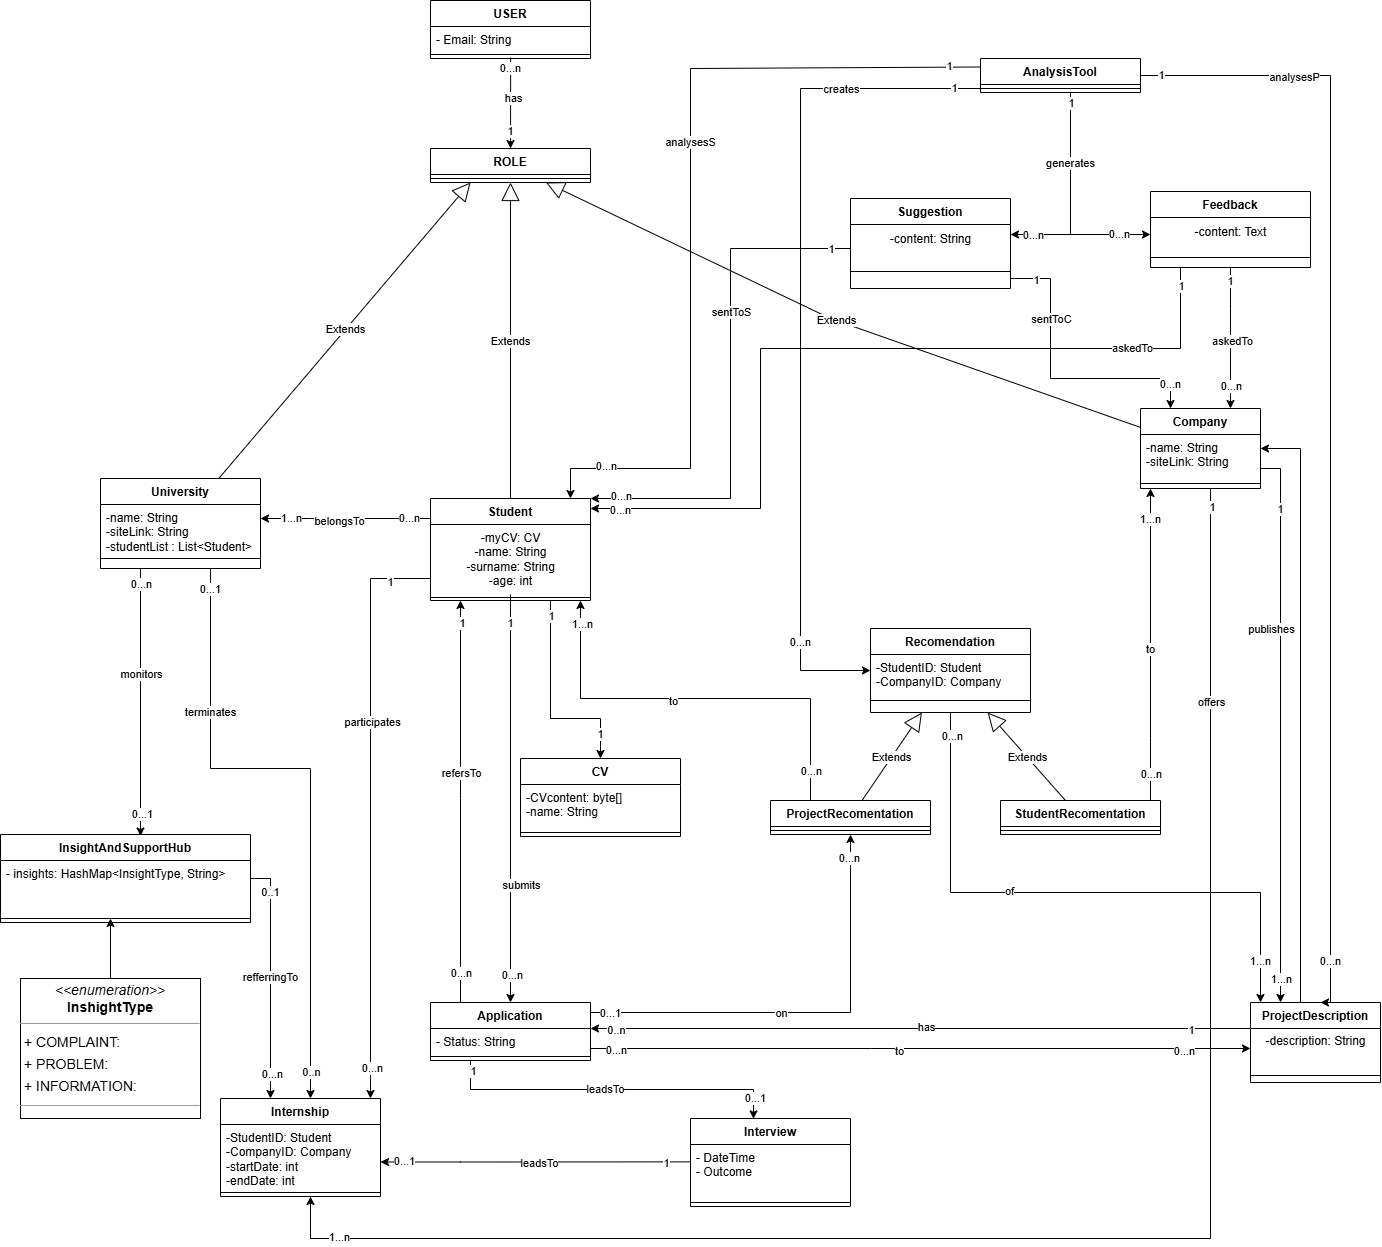
\includegraphics[width=1\linewidth]{RASD//Images/UML.drawio.png}
    \caption{Class diagram}
\end{figure}

\pagebreak
\subsection{State diagrams}
We will include some state diagrams to model the states of different objects and the transitions between these states based on events and conditions; we chose a few examples that we illustrate below.
\begin{enumerate}

\item \textbf{Recommendation process}

Entity Modeled: A recommendation generated by the platform (either for a student or a company)
This entity goes through different states throughout the usage of the platform, those states are shown here below:


\begin{figure}[H]
    \centering
    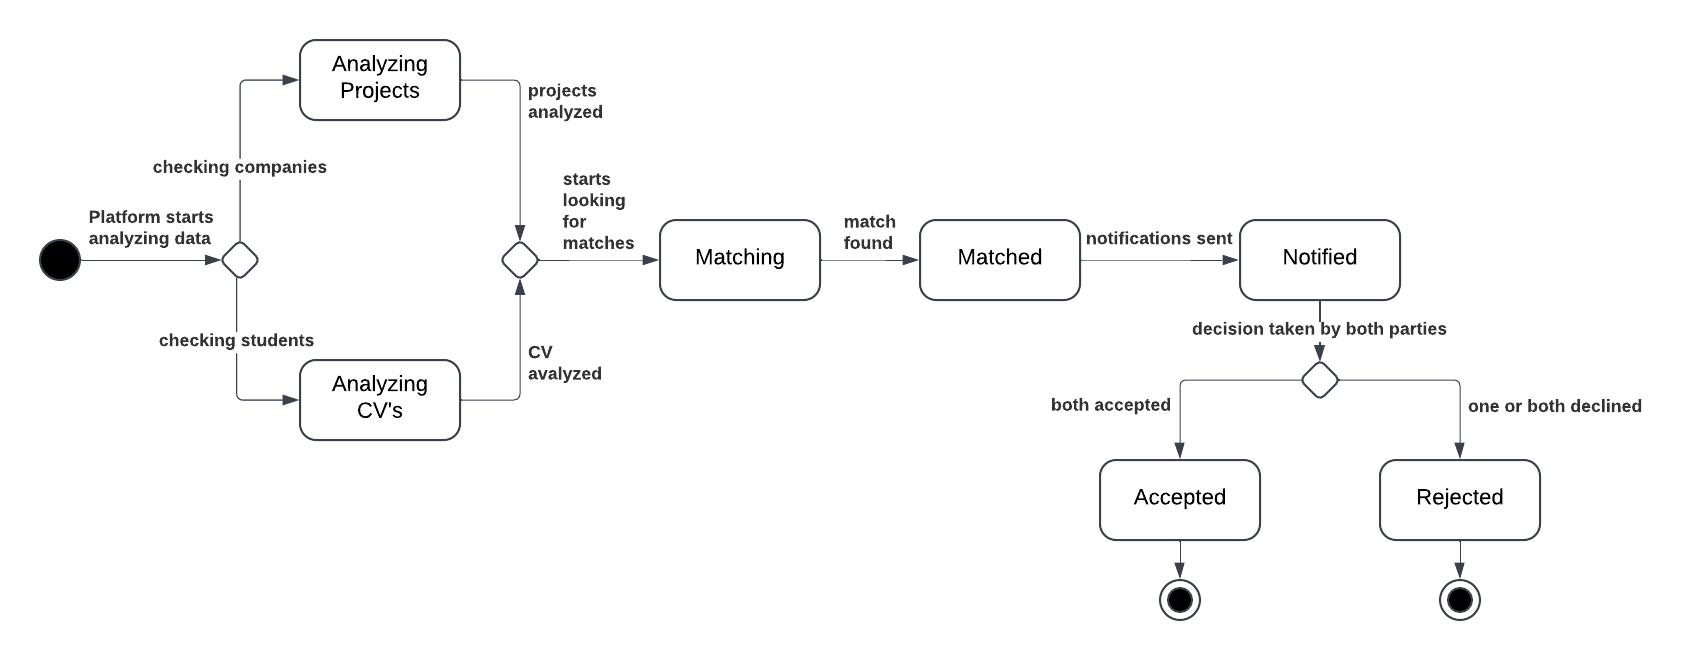
\includegraphics[width=1\linewidth]{RASD//Images/recomendation.png}
    \caption{Recommendation process}
    \label{fig:enter-label}
\end{figure}

\pagebreak
\item \textbf{Interview process}

Entity Modeled: The process of interviewing the system.
The entity we chose to model here is the interview itself since it goes through different steps based on the actions that the actors involved choose to do.

\begin{figure}[H]
    \centering
    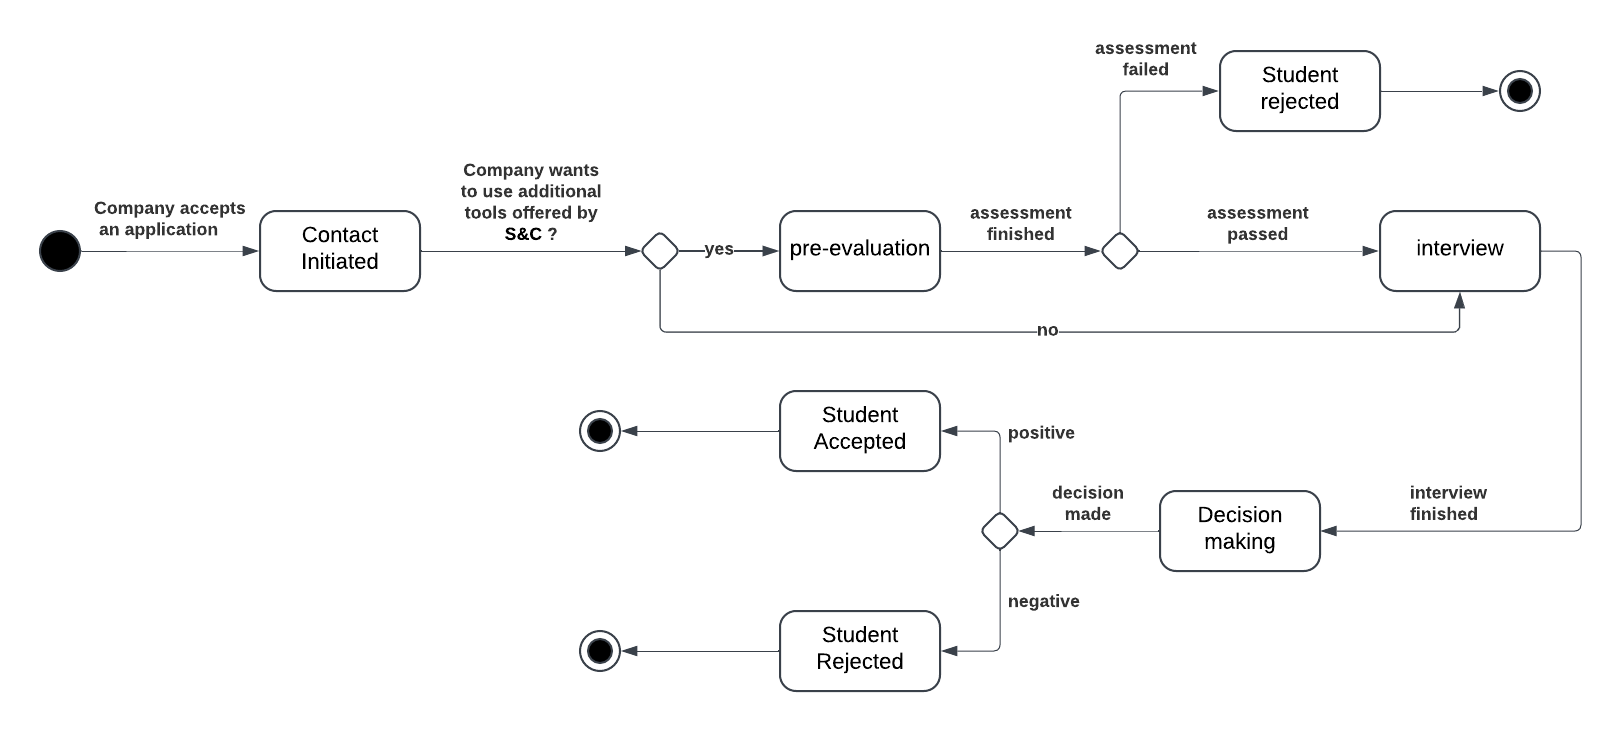
\includegraphics[width=1\linewidth]{RASD//Images/interview.png}
    \caption{Interview process}
    \label{fig:enter-label}
\end{figure}


\item \textbf{CV suggestion}

Entity Modeled: the student’s CV, which goes through different states based on the student's actions and the system's review of it.

\begin{figure}[H]
    \centering
    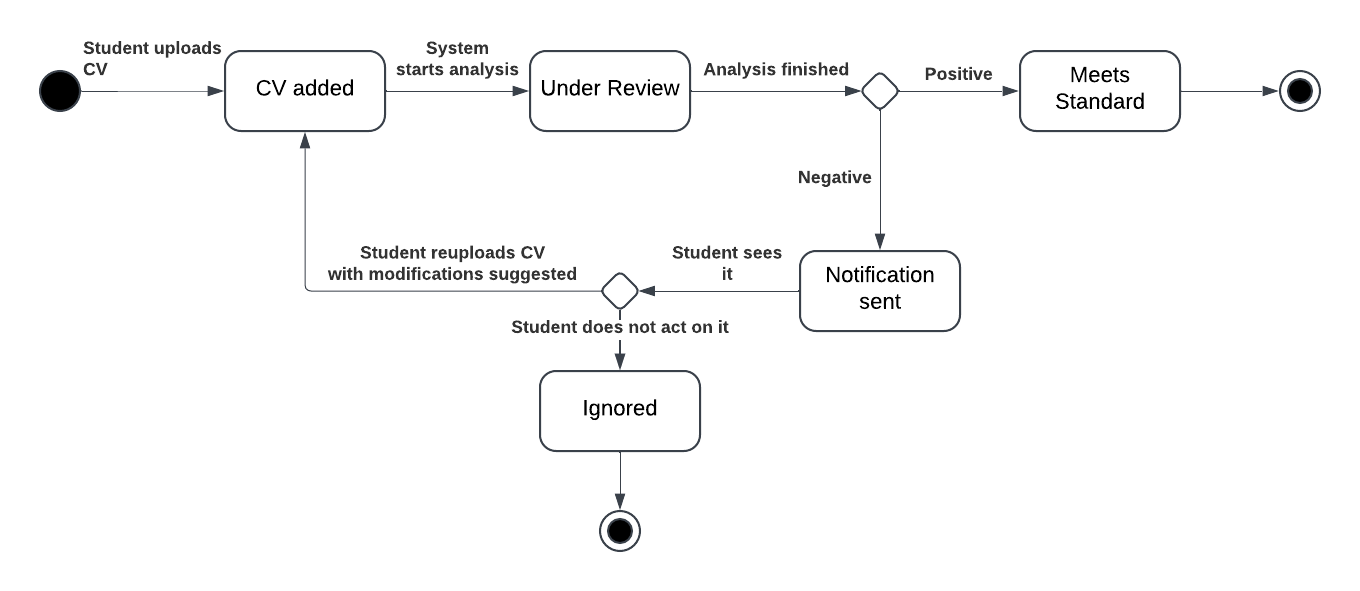
\includegraphics[width=1\linewidth]{RASD//Images/CV.png}
    \caption{CV suggestion}
    \label{fig:enter-label}
\end{figure}

\item \textbf{University handling complaints}

Entity Modeled: a complaint submitted by a student or company. The complaint goes through the following states while being published and eventually resolved:

\begin{figure}[H]
    \centering
    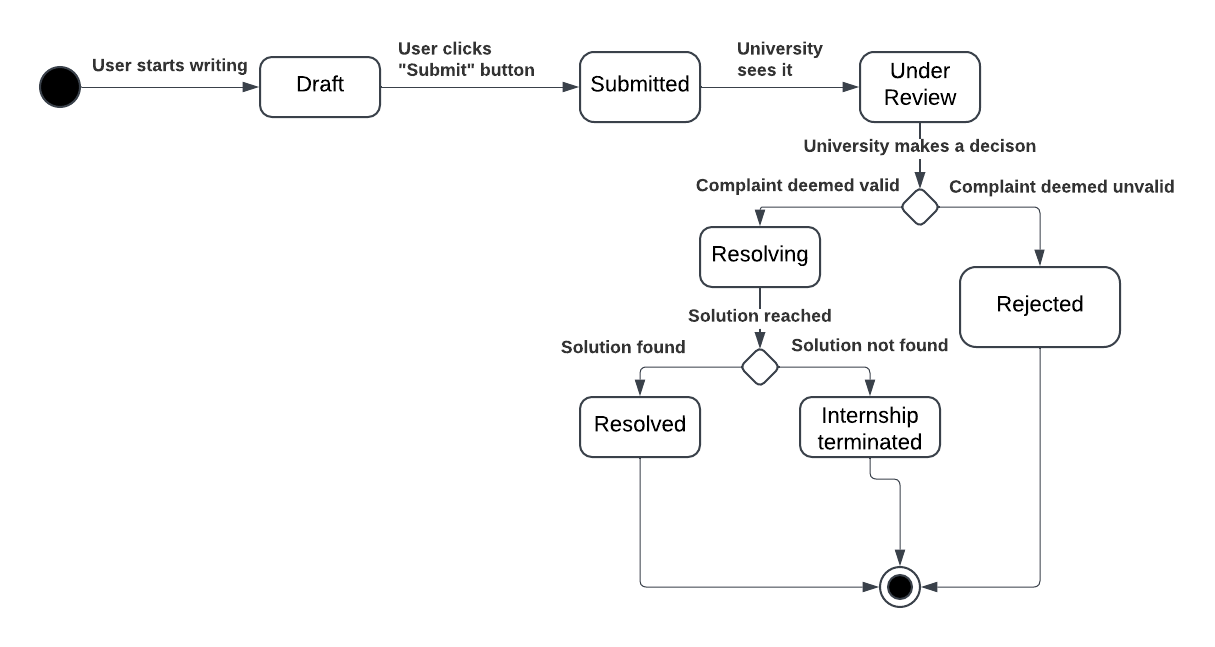
\includegraphics[width=1\linewidth]{RASD//Images/Complaints.png}
    \caption{University handling complaints}
    \label{fig:enter-label}
\end{figure}


\item \textbf{Feedback collection process}

Entity Modeled: feedback left by a user. This entity undergoes different states as shown here below: 

\begin{figure}[H]
    \centering
    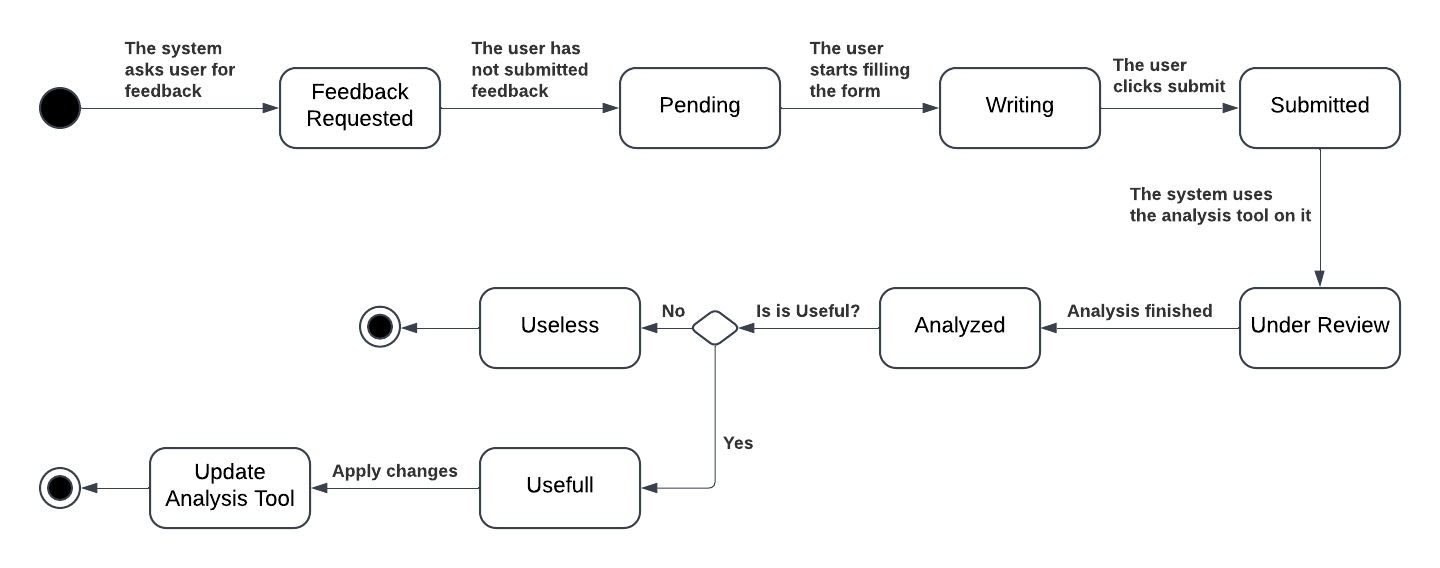
\includegraphics[width=1\linewidth]{RASD//Images/feedback2.png}
    \caption{Feedback collection process}
    \label{fig:enter-label}
\end{figure}

\end{enumerate}

\pagebreak
\section{Product Functions}

Here we will include the most important categories of use cases, so the main functions that the system should provide to its users.

\begin{enumerate}

\item \textbf{Account creation and User login}

The platform supports secure account creation for both students and company representatives. This feature ensures that only authenticated users can access the system, safeguarding personal and professional information. The user management system enables role-based access to different features.

\item \textbf{Internship posting}

Companies can post detailed descriptions of internship opportunities, including the tasks involved, required skills, application procedures, and associated benefits (e.g., mentorship, training, or compensation). The system allows companies to categorize internships by domain, location, and duration, ensuring that postings are discoverable by the most relevant candidates. By providing a structured template for submissions, the platform standardizes postings and enhances their clarity for applicants.

\item \textbf{CV analysis}

A key functionality of the platform is its automated analysis of student CVs. Using natural language processing and pattern recognition techniques, the system extracts and evaluates relevant details such as skills, academic achievements, extracurricular activities, and prior experience. This analysis facilitates the matching process by identifying the most suitable candidates for specific internships and offering students insights into how their CVs align with industry expectations.

\item \textbf{Project description analysis}

Similarly, the platform analyzes project descriptions provided by companies. This feature evaluates the scope, required skills, and potential learning outcomes of each internship project. By standardizing and comparing these descriptions, the system ensures that companies present their opportunities in the best way possible.

\pagebreak
\item \textbf{Recommendation system and statistical analysis}

One of the key features of Students\&Companies is its recommendation system, which acts like a career-matching service by connecting students with suitable internship opportunities and informing companies of potential candidates. This system operates through advanced statistical analysis methods, implementing a recommender system that uses data-driven algorithms to optimize the matching process, making it easier for students and companies to connect. 

\item \textbf{Interview and Selection management}

The platform supports the organization and management of the selection process. Companies can schedule interviews, send invitations, and manage applicant responses directly through the system. Structured tools, such as pre-defined questionnaires and assessment templates, allow companies to evaluate candidates systematically. This feature reduces administrative overhead and ensures that the selection process remains efficient and transparent.

\item \textbf{Feedback collection and analysis}

To foster continuous improvement, the platform enables users to provide feedback at various stages. Students can evaluate their internship experiences, while companies can assess the quality of applicants and their performance. This feedback is aggregated and analyzed to identify areas for improvement in the matching process, project design, and internship management.

\item \textbf{Complaint collection}

The platform includes mechanisms for students and companies to submit complaints regarding internships. Complaints may address issues such as mismatched expectations, workplace conditions, or performance concerns; this way the system ensures that all parties can voice their concerns.

\item \textbf{Internship evolution monitoring}

During the internship period, the platform facilitates the monitoring of progress. Students, companies, and universities can access tools to track progress, evaluate performance, and identify potential issues early. This feature promotes accountability and helps ensure that internships deliver meaningful outcomes for all stakeholders.

\pagebreak
\item \textbf{Complaints handling}

Universities, as key stakeholders, are responsible for resolving complaints that require intervention. The platform supports this process by providing access to all relevant data, enabling universities to make informed decisions. This feature ensures that internships adhere to agreed-upon standards and that issues are addressed to protect the interests of students and companies alike.
\end{enumerate}


\section{User charatteristic}

There are three types of registered users in S\&C: Students (STs), Companies (COMs), and Universities (UNs). Each user type has distinct characteristics and roles within the platform:

\begin{itemize}
    \item \textbf{STs}: Students use S\&C to find a company offering internships. To access the platform, they must have a device with an internet connection and an account that includes their email and personal data. Once registered, students can browse available internships, apply for them, and participate in interviews with 
    companies

    \item \textbf{COMs}:  Companies join S\&C to find students suitable for internships. To use the platform, they need a device with an internet connection and an account that includes their email and company information. Through S\&C, companies can view student applications, schedule interviews, and select candidates for internships.

    \item \textbf{UNs}: Universities that allow their students to use the Students\&Companies (S\&C) platform to find internships are provided with a dedicated institutional account. This account is typically managed by the university’s HR department or an equivalent administrative body.
    The HR department uses the account to periodically monitor the progress of internships involving their enrolled students. Through the platform, universities have access to comprehensive reports on the status of ongoing internships, including performance evaluations, feedback, and complaints submitted by either the students or the hosting companies.
    
\end{itemize}

All STs, COMs, and UNs must register with the platform to access its services. This enables seamless communication between students seeking internships, companies offering opportunities, and universities to monitor.

\pagebreak
\section{Assumptions, dependencies, constraints}
\textbf{[DA1] }Students and companies need to have a device and a reliable internet connection 

\textbf{[DA2]} Companies need to have detailed internship descriptions

\textbf{[DA3]} Students need to have a CV

\textbf{[DA4]} Students need to be enrolled at a university 

\textbf{[DA5]} Students need to create an account on S\&C as students.

\textbf{[DA6]} Companies need to create an account on S\&C as Companies.

\textbf{[DA7]} Universities need to create an account on S\&C as Universities.

\textbf{[DA8]} Companies need to be able to conduct an interview

\textbf{[DA9]} Companies need to be able to evaluate an interview

\textbf{[DA10]} Universities need to be informed about a current student's internship

\textbf{[DA11]} Universities need to be able to communicate with Students and Companies
